\documentclass[border=10pt]{standalone}
\usepackage{tikz}
\usetikzlibrary{shapes.geometric, arrows.meta, positioning, calc, backgrounds}

\begin{document}
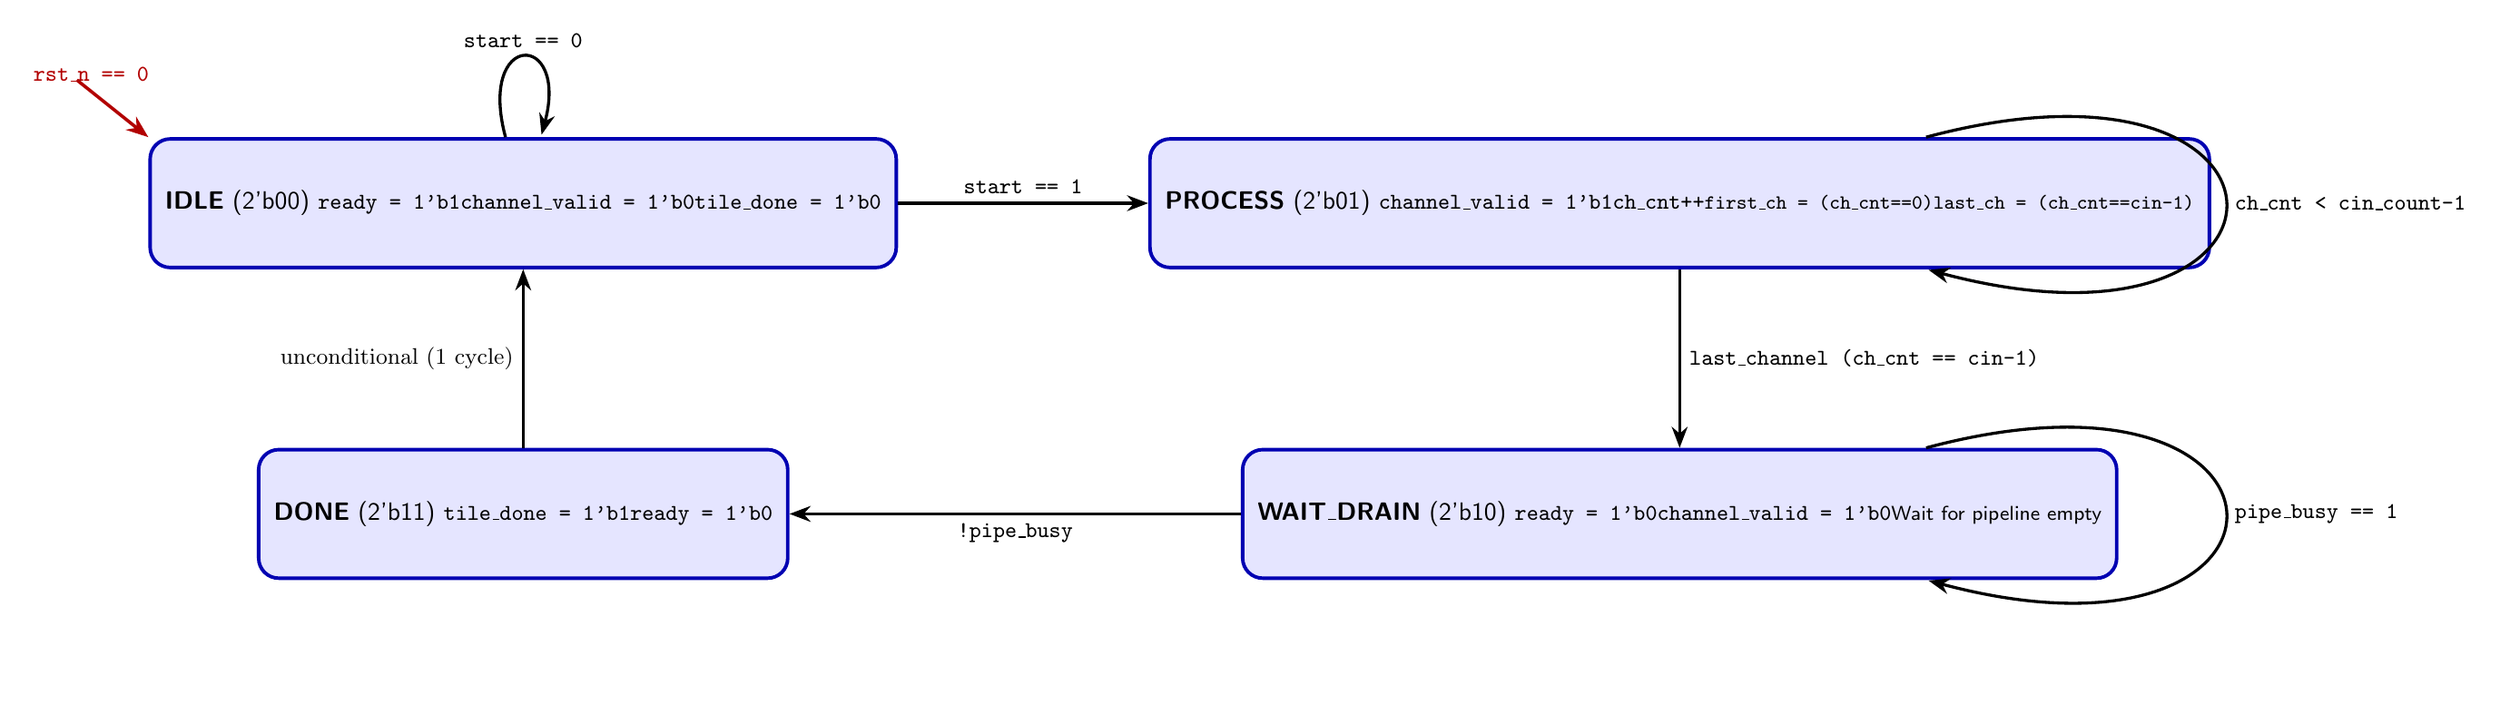
\begin{tikzpicture}[
    font=\sffamily,
    >=Stealth,
    node distance=2.5cm and 3.5cm,
    state/.style={draw=blue!70!black, fill=blue!10, line width=1.4pt, rounded corners=8pt, minimum width=3.8cm, minimum height=1.8cm, text centered, inner sep=6pt},
    trans/.style={line width=1.2pt, ->}
]

    % States
    \node[state] (idle) {
        \textbf{IDLE} (2'b00)\\
        \vspace{0.1cm}
        \small \texttt{ready = 1'b1}\\
        \small \texttt{channel\_valid = 1'b0}\\
        \small \texttt{tile\_done = 1'b0}
    };

    \node[state, right=3.5cm of idle] (process) {
        \textbf{PROCESS} (2'b01)\\
        \vspace{0.1cm}
        \small \texttt{channel\_valid = 1'b1}\\
        \small \texttt{ch\_cnt++}\\
        \footnotesize \texttt{first\_ch = (ch\_cnt==0)}\\
        \footnotesize \texttt{last\_ch = (ch\_cnt==cin-1)}
    };

    \node[state, below=2.5cm of process] (wait_drain) {
        \textbf{WAIT\_DRAIN} (2'b10)\\
        \vspace{0.1cm}
        \small \texttt{ready = 1'b0}\\
        \small \texttt{channel\_valid = 1'b0}\\
        \footnotesize Wait for pipeline empty
    };

    \node[state, below=2.5cm of idle] (done) {
        \textbf{DONE} (2'b11)\\
        \vspace{0.1cm}
        \small \texttt{tile\_done = 1'b1}\\
        \small \texttt{ready = 1'b0}
    };

    % Transitions
    \draw[trans] (idle) -- node[above, font=\small] {\texttt{start == 1}} (process);
    \draw[trans] (idle) edge[loop above] node[above, font=\small] {\texttt{start == 0}} (idle);

    \draw[trans] (process) edge[loop right] node[right, font=\small] {\texttt{ch\_cnt < cin\_count-1}} (process);
    \draw[trans] (process) -- node[right, font=\small] {\texttt{last\_channel (ch\_cnt == cin-1)}} (wait_drain);

    \draw[trans] (wait_drain) edge[loop right] node[right, font=\small] {\texttt{pipe\_busy == 1}} (wait_drain);
    \draw[trans] (wait_drain) -- node[below, font=\small] {\texttt{!pipe\_busy}} (done);

    \draw[trans] (done) -- node[left, font=\small] {unconditional (1 cycle)} (idle);

    % Reset input
    \draw[trans, red!70!black, line width=1.3pt] ($(idle.north west)+(-1, 0.8)$) -- node[pos=0.2, above, font=\small\bfseries\color{red!70!black}] {\texttt{rst\_n == 0}} (idle.north west);

\end{tikzpicture}
\end{document}
